\section{Reduction to Turing Machines}

In this section, I will reduce a Turing Machine $\langle Q, \Sigma, \Gamma, \delta, q_0, q_{halt} \rangle$ to a Colored Graph.
Instead of using actual colors, the set of colors will also contain elements like the states of the Turing Machine.
This makes it clearer which part of the Turing machine is represented by which part of the Colored Graph.
For our Colored Graph we will use the colors $\C = Q \cup \Gamma \cup \{L, R, L', R', end, end_2, end_3\}$.
I will write the name of the color next to the edges.

First, we need to encode the state of the Turing Machine.
Let $\ldots\sqcup\sqcup x_1 x_2 \ldots x_{i-1} x_{i} x_{i+1} \ldots x_k \sqcup\sqcup\ldots$ be the tape content of the Turing Machine with the head of the Turing machine pointed at $x_i$ and $q$ the current state.
Then we construct the Colored Graph as follows.

\begin{center}
    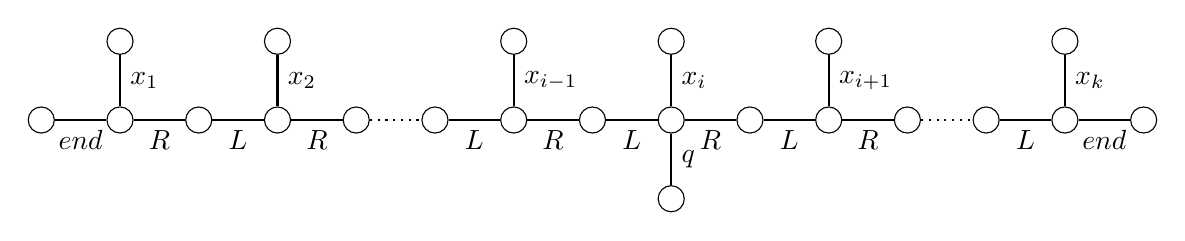
\begin{tikzpicture}
        \node[circle,draw] (A) at (1,0) {};
        \node[circle,draw] (B) at (2,0) {};
        \node[circle,draw] (Bs) at (2,1) {};
        \node[circle,draw] (C) at (3,0) {};
        \node[circle,draw] (D) at (4,0) {};
        \node[circle,draw] (Ds) at (4,1) {};
        \node[circle,draw] (E) at (5,0) {};
        \node[circle,draw] (F) at (6,0) {};
        \node[circle,draw] (G) at (7,0) {};
        \node[circle,draw] (Gs) at (7,1) {};
        \node[circle,draw] (H) at (8,0) {};
        \node[circle,draw] (I) at (9,0) {};
        \node[circle,draw] (Is) at (9,1) {};
        \node[circle,draw] (J) at (10,0) {};
        \node[circle,draw] (K) at (11,0) {};
        \node[circle,draw] (Ks) at (11,1) {};
        \node[circle,draw] (L) at (12,0) {};
        \node[circle,draw] (M) at (13,0) {};
        \node[circle,draw] (N) at (14,0) {};
        \node[circle,draw] (Ns) at (14,1) {};
        \node[circle,draw] (O) at (15,0) {};
        
        \node[circle,draw] (S) at (9,-1) {};
        \draw[thick] (S) -- node[right] {$q$} (I);
        
        \draw[thick] (A) -- node[below] {$end$} (B);
        \draw[thick] (B) -- node[right] {$x_1$} (Bs);
        \draw[thick] (B) -- node[below] {$R$} (C);
        \draw[thick] (C) -- node[below] {$L$} (D);
        \draw[thick] (D) -- node[right] {$x_2$} (Ds);
        \draw[thick] (D) -- node[below] {$R$} (E);
        \draw[thick, dotted] (E) -- node[below] {} (F);
        \draw[thick] (F) -- node[below] {$L$} (G);
        \draw[thick] (G) -- node[below] {$R$} (H);
        \draw[thick] (G) -- node[right] {$x_{i-1}$} (Gs);
        \draw[thick] (H) -- node[below] {$L$} (I);
        \draw[thick] (I) -- node[right] {$x_i$} (Is);
        \draw[thick] (I) -- node[below] {$R$} (J);
        \draw[thick] (J) -- node[below] {$L$} (K);
        \draw[thick] (K) -- node[right] {$x_{i+1}$} (Ks);
        \draw[thick] (K) -- node[below] {$R$} (L);
        \draw[thick, dotted] (L) -- node[below] {} (M);
        \draw[thick] (M) -- node[below] {$L$} (N);
        \draw[thick] (N) -- node[right] {$x_k$} (Ns);
        \draw[thick] (N) -- node[below] {$end$} (O);
    \end{tikzpicture}
\end{center}

To avoid handling multiple special cases we will also make sure that the Colored Graph always has at least two cells of the Turing machine.
So even for an empty tape we have two cells that are simply marked with the placeholder symbol $\sqcup$.

The rules to emulate the Turing Machine are as follows.

\begin{itemize}
    \item For each transition $\delta(q, x) = (q', y, R)$ we add the following rule.
    \begin{center}
        \begin{tikzpicture}
        \begin{scope}[xshift=-2cm]
            \node[circle,draw,fill] (A) at (0, 0) {};
            \node[circle,draw] (B) at (-1,0) {};
            \node[circle,draw] (C) at (0,1) {};
            \node[circle,draw] (D) at (1,0) {};
            \node[circle,draw] (E) at (0,-1) {};
            
            \draw[thick] (A) -- node[below] {$L$} (B);
            \draw[thick] (A) -- node[right] {$x$} (C);
            \draw[thick] (A) -- node[below] {$R$} (D);
            \draw[thick] (A) -- node[right] {$q$} (E);
        \end{scope}
    
        \draw [line width=1pt, double distance=3pt, arrows = {-Latex[length=0pt 3 0]}] (-0.5,0) -- node[above] {(1)} (0.5,0);
        
        \begin{scope}[xshift=2cm]
            \node[circle,draw,fill] (A) at (0, 0) {};
            \node[circle,draw,fill] (A') at (1, -1) {};
            \node[circle,draw] (B) at (-1,0) {};
            \node[circle,draw] (C) at (0,1) {};
            \node[circle,draw] (D) at (1,0) {};
            \node[circle,draw] (E) at (0,-1) {};

            \draw[thick] (A) -- node[below] {$L$} (B);
            \draw[thick] (A) -- node[right] {$y$} (C);
            \draw[thick] (A) -- node[below] {$R'$} (D);
            \draw[thick] (A') -- node[right] {$q'$} (D);
        \end{scope}
        \end{tikzpicture}
    \end{center}
    \item For each transition $\delta(q, x) = (q', y, L)$ we add the following rule.
    \begin{center}
        \begin{tikzpicture}
        \begin{scope}[xshift=-2cm]
            \node[circle,draw,fill] (A) at (0, 0) {};
            \node[circle,draw] (B) at (-1,0) {};
            \node[circle,draw] (C) at (0,1) {};
            \node[circle,draw] (D) at (1,0) {};
            \node[circle,draw] (E) at (0,-1) {};
            
            \draw[thick] (A) -- node[below] {$L$} (B);
            \draw[thick] (A) -- node[right] {$x$} (C);
            \draw[thick] (A) -- node[below] {$R$} (D);
            \draw[thick] (A) -- node[right] {$q$} (E);
        \end{scope}
    
        \draw [line width=1pt, double distance=3pt, arrows = {-Latex[length=0pt 3 0]}] (-0.5,0) -- node[above] {(2)} (0.5,0);
        
        \begin{scope}[xshift=2cm]
            \node[circle,draw,fill] (A) at (0, 0) {};
            \node[circle,draw,fill] (A') at (-1, -1) {};
            \node[circle,draw] (B) at (-1,0) {};
            \node[circle,draw] (C) at (0,1) {};
            \node[circle,draw] (D) at (1,0) {};
            \node[circle,draw] (E) at (0,-1) {};

            \draw[thick] (A) -- node[below] {$L'$} (B);
            \draw[thick] (A) -- node[right] {$y$} (C);
            \draw[thick] (A) -- node[below] {$R$} (D);
            \draw[thick] (A') -- node[left] {$q'$} (B);
        \end{scope}
        \end{tikzpicture}
    \end{center}
    \item Next for each $q \in Q$ we add the following two rules.
    \begin{center}
        \begin{tikzpicture}
        \begin{scope}[xshift=-4cm]
            \begin{scope}[xshift=-2cm]
                \node[circle,draw,fill] (A) at (0, 0) {};
                \node[circle,draw] (B) at (-1,0) {};
                \node[circle,draw] (D) at (1,0) {};
                \node[circle,draw] (E) at (0,-1) {};
                
                \draw[thick] (A) -- node[below] {$R'$} (B);
                \draw[thick] (A) -- node[below] {$L$} (D);
                \draw[thick] (A) -- node[right] {$q$} (E);
            \end{scope}
        
            \draw [line width=1pt, double distance=3pt, arrows = {-Latex[length=0pt 3 0]}] (-0.5,0) -- node[above] {(3)} (0.5,0);
            
            \begin{scope}[xshift=2cm]
                \node[circle,draw,fill] (A) at (0, 0) {};
                \node[circle,draw,fill] (A') at (1, -1) {};
                \node[circle,draw] (B) at (-1,0) {};
                \node[circle,draw] (D) at (1,0) {};
                \node[circle,draw] (E) at (0,-1) {};
    
                \draw[thick] (A) -- node[below] {$R$} (B);
                \draw[thick] (A) -- node[below] {$L$} (D);
                \draw[thick] (A') -- node[right] {$q$} (D);
            \end{scope}
        \end{scope}

        \begin{scope}[xshift=4cm]
            \begin{scope}[xshift=-2cm]
                \node[circle,draw,fill] (A) at (0, 0) {};
                \node[circle,draw] (B) at (-1,0) {};
                \node[circle,draw] (D) at (1,0) {};
                \node[circle,draw] (E) at (0,-1) {};
                
                \draw[thick] (A) -- node[below] {$R$} (B);
                \draw[thick] (A) -- node[below] {$L'$} (D);
                \draw[thick] (A) -- node[left] {$q$} (E);
            \end{scope}
        
            \draw [line width=1pt, double distance=3pt, arrows = {-Latex[length=0pt 3 0]}] (-0.5,0) -- node[above] {(4)} (0.5,0);
            
            \begin{scope}[xshift=2cm]
                \node[circle,draw,fill] (A) at (0, 0) {};
                \node[circle,draw,fill] (A') at (-1, -1) {};
                \node[circle,draw] (B) at (-1,0) {};
                \node[circle,draw] (D) at (1,0) {};
                \node[circle,draw] (E) at (0,-1) {};
    
                \draw[thick] (A) -- node[below] {$R$} (B);
                \draw[thick] (A) -- node[below] {$L$} (D);
                \draw[thick] (A') -- node[left] {$q$} (B);
            \end{scope}
        \end{scope}
        \end{tikzpicture}
    \end{center}
    \item Since we create isolated vertices with some rules, we add a Delete Rule that just deletes such vertices.
    \begin{center}
        \begin{tikzpicture}
        \begin{scope}[xshift=-1.5cm]
            \node[circle,draw,fill] (A) at (0, 0) {};
        \end{scope}
    
        \draw [line width=1pt, double distance=3pt, arrows = {-Latex[length=0pt 3 0]}] (-0.5,0) -- node[above] {(5)} (0.5,0);
        
        \begin{scope}[xshift=2cm]
        \end{scope}
        \end{tikzpicture}
    \end{center}
\end{itemize}

There are still 6 rules missing to deal with the edge of the tape, but these rules alone can simulate a transition of the Turing machine.
So before introducing the remaining rules let's first see an example transition.
For this we will only look at the relavent section of the Turing machine where the head is currently pointing to.
Assume we have a transition $\delta(q, x) = (q', y, R)$.
Then the Colored graph will evolve as follows where I will always mark the node a rule will be applied to in the next step with black.

\begin{center}
    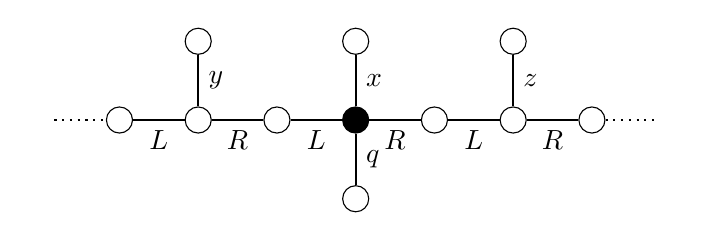
\begin{tikzpicture}
        \node[circle] (E) at (5,0) {};
        \node[circle,draw] (F) at (6,0) {};
        \node[circle,draw] (G) at (7,0) {};
        \node[circle,draw] (Gs) at (7,1) {};
        \node[circle,draw] (H) at (8,0) {};
        \node[circle,draw,fill] (I) at (9,0) {};
        \node[circle,draw] (Is) at (9,1) {};
        \node[circle,draw] (J) at (10,0) {};
        \node[circle,draw] (K) at (11,0) {};
        \node[circle,draw] (Ks) at (11,1) {};
        \node[circle,draw] (L) at (12,0) {};
        \node[circle] (M) at (13,0) {};
        
        \node[circle,draw] (S) at (9,-1) {};
        \draw[thick] (S) -- node[right] {$q$} (I);
        
        \draw[thick, dotted] (E) -- node[below] {} (F);
        \draw[thick] (F) -- node[below] {$L$} (G);
        \draw[thick] (G) -- node[right] {$y$} (Gs);
        \draw[thick] (G) -- node[below] {$R$} (H);
        \draw[thick] (H) -- node[below] {$L$} (I);
        \draw[thick] (I) -- node[right] {$x$} (Is);
        \draw[thick] (I) -- node[below] {$R$} (J);
        \draw[thick] (J) -- node[below] {$L$} (K);
        \draw[thick] (K) -- node[right] {$z$} (Ks);
        \draw[thick] (K) -- node[below] {$R$} (L);
        \draw[thick, dotted] (L) -- node[below] {} (M);
    \end{tikzpicture}
\end{center}

First, the node the head is pointing to is the only node that a rule can be applied to so rule (1) will be applied to it.

\begin{center}
    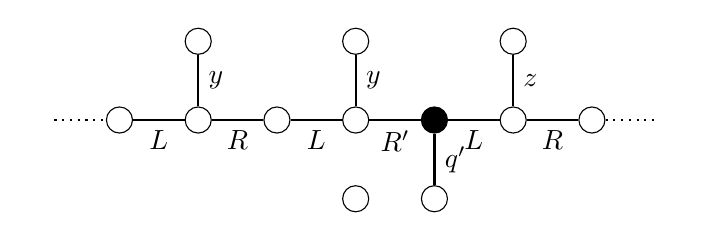
\begin{tikzpicture}
        \node[circle] (E) at (5,0) {};
        \node[circle,draw] (F) at (6,0) {};
        \node[circle,draw] (G) at (7,0) {};
        \node[circle,draw] (Gs) at (7,1) {};
        \node[circle,draw] (H) at (8,0) {};
        \node[circle,draw] (I) at (9,0) {};
        \node[circle,draw] (Is) at (9,1) {};
        \node[circle,draw,fill] (J) at (10,0) {};
        \node[circle,draw] (K) at (11,0) {};
        \node[circle,draw] (Ks) at (11,1) {};
        \node[circle,draw] (L) at (12,0) {};
        \node[circle] (M) at (13,0) {};
        
        \node[circle,draw] (S') at (9,-1) {};
        \node[circle,draw] (S) at (10,-1) {};
        \draw[thick] (S) -- node[right] {$q'$} (J);
        
        \draw[thick, dotted] (E) -- node[below] {} (F);
        \draw[thick] (F) -- node[below] {$L$} (G);
        \draw[thick] (G) -- node[right] {$y$} (Gs);
        \draw[thick] (G) -- node[below] {$R$} (H);
        \draw[thick] (H) -- node[below] {$L$} (I);
        \draw[thick] (I) -- node[right] {$y$} (Is);
        \draw[thick] (I) -- node[below] {$R'$} (J);
        \draw[thick] (J) -- node[below] {$L$} (K);
        \draw[thick] (K) -- node[right] {$z$} (Ks);
        \draw[thick] (K) -- node[below] {$R$} (L);
        \draw[thick, dotted] (L) -- node[below] {} (M);
    \end{tikzpicture}
\end{center}

Now we can either apply rule (5) to the isolated vertex or rule (3) to the node marked in black.
Since these nodes are disconnected it is clear that the order of application does not matter.
Here, we will apply rule (3) first resulting in the following.

\begin{center}
    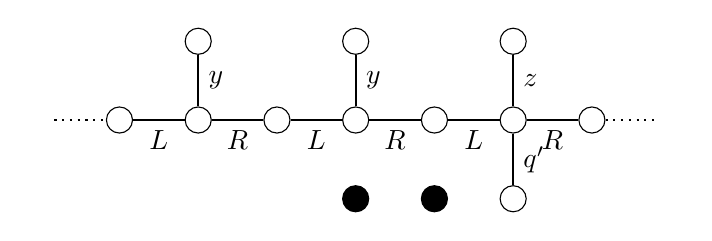
\begin{tikzpicture}
        \node[circle] (E) at (5,0) {};
        \node[circle,draw] (F) at (6,0) {};
        \node[circle,draw] (G) at (7,0) {};
        \node[circle,draw] (Gs) at (7,1) {};
        \node[circle,draw] (H) at (8,0) {};
        \node[circle,draw] (I) at (9,0) {};
        \node[circle,draw] (Is) at (9,1) {};
        \node[circle,draw] (J) at (10,0) {};
        \node[circle,draw] (K) at (11,0) {};
        \node[circle,draw] (Ks) at (11,1) {};
        \node[circle,draw] (L) at (12,0) {};
        \node[circle] (M) at (13,0) {};
        
        \node[circle,draw,fill] (S') at (9,-1) {};
        \node[circle,draw,fill] (S'') at (10,-1) {};
        \node[circle,draw] (S) at (11,-1) {};
        \draw[thick] (S) -- node[right] {$q'$} (K);
        
        \draw[thick, dotted] (E) -- node[below] {} (F);
        \draw[thick] (F) -- node[below] {$L$} (G);
        \draw[thick] (G) -- node[right] {$y$} (Gs);
        \draw[thick] (G) -- node[below] {$R$} (H);
        \draw[thick] (H) -- node[below] {$L$} (I);
        \draw[thick] (I) -- node[right] {$y$} (Is);
        \draw[thick] (I) -- node[below] {$R$} (J);
        \draw[thick] (J) -- node[below] {$L$} (K);
        \draw[thick] (K) -- node[right] {$z$} (Ks);
        \draw[thick] (K) -- node[below] {$R$} (L);
        \draw[thick, dotted] (L) -- node[below] {} (M);
    \end{tikzpicture}
\end{center}

With two applications of rule (5) we can delete the isolated vertices and complete the Turing machine transition.
Of course the rules for the next transition could also already be applied but the isolated will be deleted eventually as long as the Turing machine terminates and otherwise thay have no influence on the the rest of the graph.

\begin{center}
    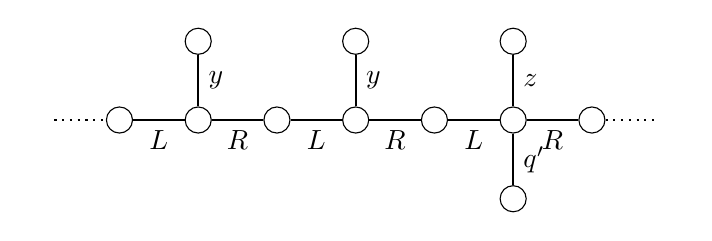
\begin{tikzpicture}
        \node[circle] (E) at (5,0) {};
        \node[circle,draw] (F) at (6,0) {};
        \node[circle,draw] (G) at (7,0) {};
        \node[circle,draw] (Gs) at (7,1) {};
        \node[circle,draw] (H) at (8,0) {};
        \node[circle,draw] (I) at (9,0) {};
        \node[circle,draw] (Is) at (9,1) {};
        \node[circle,draw] (J) at (10,0) {};
        \node[circle,draw] (K) at (11,0) {};
        \node[circle,draw] (Ks) at (11,1) {};
        \node[circle,draw] (L) at (12,0) {};
        \node[circle] (M) at (13,0) {};

        \node[circle,draw] (S) at (11,-1) {};
        \draw[thick] (S) -- node[right] {$q'$} (K);
        
        \draw[thick, dotted] (E) -- node[below] {} (F);
        \draw[thick] (F) -- node[below] {$L$} (G);
        \draw[thick] (G) -- node[right] {$y$} (Gs);
        \draw[thick] (G) -- node[below] {$R$} (H);
        \draw[thick] (H) -- node[below] {$L$} (I);
        \draw[thick] (I) -- node[right] {$y$} (Is);
        \draw[thick] (I) -- node[below] {$R$} (J);
        \draw[thick] (J) -- node[below] {$L$} (K);
        \draw[thick] (K) -- node[right] {$z$} (Ks);
        \draw[thick] (K) -- node[below] {$R$} (L);
        \draw[thick, dotted] (L) -- node[below] {} (M);
    \end{tikzpicture}
\end{center}

A transition that moves the head to the left can similarly be simulated by rules (2) and (4).

What's left to perform a complete simulation of t Turing machine is handling the edges of the tape.
For this we will add rules that extend the tape once the head reaches them.
Note that it is important to only extend the tape once the head actually reaches them, otherwise they could be extended indefinetly and the reduction of the Colored graph would not terminate.
For each $x \in \Gamma$ and $q \in Q$ we add the following rules.

\begin{center}
    \begin{tikzpicture}
    \begin{scope}[xshift=-4cm]
        \begin{scope}[xshift=-2cm]
            \node[circle,draw,fill] (A) at (0, 0) {};
            \node[circle,draw] (B) at (-1,0) {};
            \node[circle,draw] (C) at (0,1) {};
            \node[circle,draw] (D) at (1,0) {};
            \node[circle,draw] (E) at (0,-1) {};
            
            \draw[thick] (A) -- node[right] {$x$} (C);
            \draw[thick] (A) -- node[right] {$q$} (E);
            \draw[thick] (A) -- node[below] {$end$} (B);
            \draw[thick] (A) -- node[below] {$R$} (D);
        \end{scope}
    
        \draw [line width=1pt, double distance=3pt, arrows = {-Latex[length=0pt 3 0]}] (-0.5,0) -- node[above] {(6)} (0.5,0);
        
        \begin{scope}[xshift=3cm]
            \node[circle,draw,fill] (A) at (0, 0) {};
            \node[circle,draw,fill] (A') at (-2, 0) {};
            \node[circle,draw] (B) at (-1,0) {};
            \node[circle,draw] (C) at (0,1) {};
            \node[circle,draw] (D) at (1,0) {};
            \node[circle,draw] (E) at (0,-1) {};
            
            \draw[thick] (A) -- node[right] {$x$} (C);
            \draw[thick] (A) -- node[right] {$q$} (E);
            \draw[thick] (A) -- node[below] {$end_2$} (B);
            \draw[thick] (A) -- node[below] {$R$} (D);
            \draw[thick] (A') -- node[below] {$R$} (B);
        \end{scope}
    \end{scope}

    \begin{scope}[xshift=4cm]
        \begin{scope}[xshift=-2cm]
            \node[circle,draw,fill] (A) at (0, 0) {};
            \node[circle,draw] (B) at (-1,0) {};
            \node[circle,draw] (C) at (0,1) {};
            \node[circle,draw] (D) at (1,0) {};
            \node[circle,draw] (E) at (0,-1) {};
            
            \draw[thick] (A) -- node[right] {$x$} (C);
            \draw[thick] (A) -- node[right] {$q$} (E);
            \draw[thick] (A) -- node[below] {$L$} (B);
            \draw[thick] (A) -- node[below] {$end$} (D);
        \end{scope}
    
        \draw [line width=1pt, double distance=3pt, arrows = {-Latex[length=0pt 3 0]}] (-0.5,0) -- node[above] {(9)} (0.5,0);
        
        \begin{scope}[xshift=2cm]
            \node[circle,draw,fill] (A) at (0, 0) {};
            \node[circle,draw,fill] (A') at (2, 0) {};
            \node[circle,draw] (B) at (-1,0) {};
            \node[circle,draw] (C) at (0,1) {};
            \node[circle,draw] (D) at (1,0) {};
            \node[circle,draw] (E) at (0,-1) {};
            
            \draw[thick] (A) -- node[right] {$x$} (C);
            \draw[thick] (A) -- node[right] {$q$} (E);
            \draw[thick] (A) -- node[below] {$L$} (B);
            \draw[thick] (A) -- node[below] {$end_2$} (D);
            \draw[thick] (A') -- node[below] {$L$} (D);
        \end{scope}
    \end{scope}
    \end{tikzpicture}

    \begin{tikzpicture}
        \begin{scope}[xshift=-4cm]
            \begin{scope}[xshift=-2cm]
                \node[circle,draw,fill] (A) at (0, 0) {};
                \node[circle,draw] (B) at (-1,0) {};
                \node[circle,draw] (D) at (1,0) {};
                
                \draw[thick] (A) -- node[below] {$R$} (B);
                \draw[thick] (A) -- node[below] {$end_2$} (D);
            \end{scope}
        
            \draw [line width=1pt, double distance=3pt, arrows = {-Latex[length=0pt 3 0]}] (-0.5,0) -- node[above] {(7)} (0.5,0);
            
            \begin{scope}[xshift=2cm]
                \node[circle,draw,fill] (A) at (0, 0) {};
                \node[circle,draw,fill] (A') at (-1, 1) {};
                \node[circle,draw] (B) at (-1,0) {};
                \node[circle,draw] (D) at (1,0) {};
                
                \draw[thick] (A) -- node[below] {$R$} (B);
                \draw[thick] (A) -- node[below] {$end_3$} (D);
                \draw[thick] (A') -- node[left] {$\sqcup$} (B);
            \end{scope}
        \end{scope}

        \begin{scope}[xshift=4cm]
            \begin{scope}[xshift=-2cm]
                \node[circle,draw,fill] (A) at (0, 0) {};
                \node[circle,draw] (B) at (-1,0) {};
                \node[circle,draw] (D) at (1,0) {};
                
                \draw[thick] (A) -- node[below] {$end_2$} (B);
                \draw[thick] (A) -- node[below] {$L$} (D);
            \end{scope}
        
            \draw [line width=1pt, double distance=3pt, arrows = {-Latex[length=0pt 3 0]}] (-0.5,0) -- node[above] {(10)} (0.5,0);
            
            \begin{scope}[xshift=2cm]
                \node[circle,draw,fill] (A) at (0, 0) {};
                \node[circle,draw,fill] (A') at (1, 1) {};
                \node[circle,draw] (B) at (-1,0) {};
                \node[circle,draw] (D) at (1,0) {};
                
                \draw[thick] (A) -- node[below] {$end_3$} (B);
                \draw[thick] (A) -- node[below] {$L$} (D);
                \draw[thick] (A') -- node[left] {$\sqcup$} (D);
            \end{scope}
        \end{scope}
        \end{tikzpicture}

        \vspace*{0.8cm}

        \begin{tikzpicture}
            \begin{scope}[xshift=-4cm]
                \begin{scope}[xshift=-2cm]
                    \node[circle,draw,fill] (A) at (0, 0) {};
                    \node[circle,draw] (B) at (-1,0) {};
                    \node[circle,draw] (D) at (1,0) {};
                    
                    \draw[thick] (A) -- node[below] {$R$} (B);
                    \draw[thick] (A) -- node[below] {$end_3$} (D);
                \end{scope}
            
                \draw [line width=1pt, double distance=3pt, arrows = {-Latex[length=0pt 3 0]}] (-0.5,0) -- node[above] {(8)} (0.5,0);
                
                \begin{scope}[xshift=3cm]
                    \node[circle,draw,fill] (A) at (0, 0) {};
                    \node[circle,draw,fill] (A') at (-2, 0) {};
                    \node[circle,draw] (B) at (-1,0) {};
                    \node[circle,draw] (D) at (1,0) {};
                    
                    \draw[thick] (A) -- node[below] {$R$} (B);
                    \draw[thick] (A) -- node[below] {$L$} (D);
                    \draw[thick] (A') -- node[below] {$end$} (B);
                \end{scope}
            \end{scope}
    
            \begin{scope}[xshift=4cm]
                \begin{scope}[xshift=-2cm]
                    \node[circle,draw,fill] (A) at (0, 0) {};
                    \node[circle,draw] (B) at (-1,0) {};
                    \node[circle,draw] (D) at (1,0) {};
                    
                    \draw[thick] (A) -- node[below] {$end_3$} (B);
                    \draw[thick] (A) -- node[below] {$L$} (D);
                \end{scope}
            
                \draw [line width=1pt, double distance=3pt, arrows = {-Latex[length=0pt 3 0]}] (-0.5,0) -- node[above] {(11)} (0.5,0);
                
                \begin{scope}[xshift=2cm]
                    \node[circle,draw,fill] (A) at (0, 0) {};
                    \node[circle,draw,fill] (A') at (2, 0) {};
                    \node[circle,draw] (B) at (-1,0) {};
                    \node[circle,draw] (D) at (1,0) {};
                    
                    \draw[thick] (A) -- node[below] {$R$} (B);
                    \draw[thick] (A) -- node[below] {$L$} (D);
                    \draw[thick] (A') -- node[below] {$end$} (D);
                \end{scope}
            \end{scope}
        \end{tikzpicture}
\end{center}

The extension of the tape will be handled in states as we need to add multiple nodes.
The stages are marked with the $end_i$ colors.
First when the head hits one of the tape borders, we add a new node to that side.
Then we add the placeholder $\sqcup$ to that new node.
Finally we add a new node that marks the new end of the tape.
An example entension of the left side of the tape would look at follows, where we apply rule (6), (7) and (8) in that order.

\begin{center}
    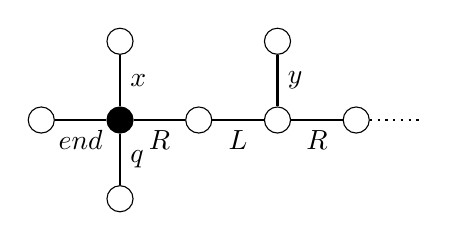
\begin{tikzpicture}
        \node[circle,draw] (A) at (1,0) {};
        \node[circle,draw,fill] (B) at (2,0) {};
        \node[circle,draw] (Bs) at (2,1) {};
        \node[circle,draw] (C) at (3,0) {};
        \node[circle,draw] (D) at (4,0) {};
        \node[circle,draw] (Ds) at (4,1) {};
        \node[circle,draw] (E) at (5,0) {};
        \node[circle] (F) at (6,0) {};
        
        \node[circle,draw] (S) at (2,-1) {};
        \draw[thick] (S) -- node[right] {$q$} (B);
        
        \draw[thick] (A) -- node[below] {$end$} (B);
        \draw[thick] (B) -- node[right] {$x$} (Bs);
        \draw[thick] (B) -- node[below] {$R$} (C);
        \draw[thick] (C) -- node[below] {$L$} (D);
        \draw[thick] (D) -- node[right] {$y$} (Ds);
        \draw[thick] (D) -- node[below] {$R$} (E);
        \draw[thick, dotted] (E) -- node[below] {} (F);
    \end{tikzpicture}
\end{center}

\begin{center}
    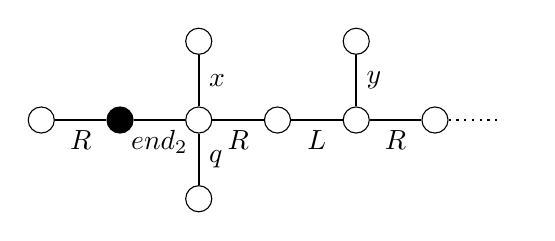
\begin{tikzpicture}
        \node[circle,draw] (N) at (0,0) {};
        \node[circle,draw,fill] (A) at (1,0) {};
        \node[circle,draw] (B) at (2,0) {};
        \node[circle,draw] (Bs) at (2,1) {};
        \node[circle,draw] (C) at (3,0) {};
        \node[circle,draw] (D) at (4,0) {};
        \node[circle,draw] (Ds) at (4,1) {};
        \node[circle,draw] (E) at (5,0) {};
        \node[circle] (F) at (6,0) {};
        
        \node[circle,draw] (S) at (2,-1) {};
        \draw[thick] (S) -- node[right] {$q$} (B);
        
        \draw[thick] (N) -- node[below] {$R$} (A);
        \draw[thick] (A) -- node[below] {$end_2$} (B);
        \draw[thick] (B) -- node[right] {$x$} (Bs);
        \draw[thick] (B) -- node[below] {$R$} (C);
        \draw[thick] (C) -- node[below] {$L$} (D);
        \draw[thick] (D) -- node[right] {$y$} (Ds);
        \draw[thick] (D) -- node[below] {$R$} (E);
        \draw[thick, dotted] (E) -- node[below] {} (F);
    \end{tikzpicture}
\end{center}

\begin{center}
    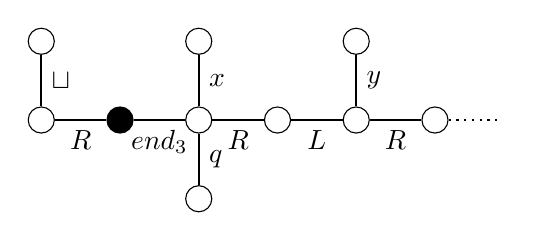
\begin{tikzpicture}
        \node[circle,draw] (N) at (0,0) {};
        \node[circle,draw] (Ns) at (0,1) {};
        \node[circle,draw,fill] (A) at (1,0) {};
        \node[circle,draw] (B) at (2,0) {};
        \node[circle,draw] (Bs) at (2,1) {};
        \node[circle,draw] (C) at (3,0) {};
        \node[circle,draw] (D) at (4,0) {};
        \node[circle,draw] (Ds) at (4,1) {};
        \node[circle,draw] (E) at (5,0) {};
        \node[circle] (F) at (6,0) {};
        
        \node[circle,draw] (S) at (2,-1) {};
        \draw[thick] (S) -- node[right] {$q$} (B);
        
        \draw[thick] (N) -- node[below] {$R$} (A);
        \draw[thick] (N) -- node[right] {$\sqcup$} (Ns);
        \draw[thick] (A) -- node[below] {$end_3$} (B);
        \draw[thick] (B) -- node[right] {$x$} (Bs);
        \draw[thick] (B) -- node[below] {$R$} (C);
        \draw[thick] (C) -- node[below] {$L$} (D);
        \draw[thick] (D) -- node[right] {$y$} (Ds);
        \draw[thick] (D) -- node[below] {$R$} (E);
        \draw[thick, dotted] (E) -- node[below] {} (F);
    \end{tikzpicture}
\end{center}

\begin{center}
    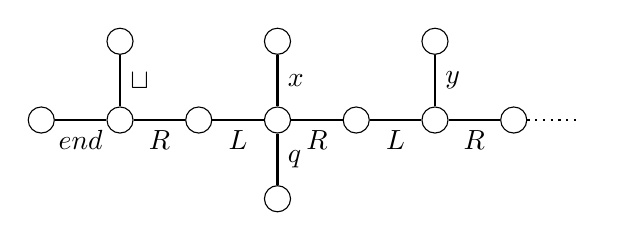
\begin{tikzpicture}
        \node[circle,draw] (M) at (-1,0) {};
        \node[circle,draw] (N) at (0,0) {};
        \node[circle,draw] (Ns) at (0,1) {};
        \node[circle,draw] (A) at (1,0) {};
        \node[circle,draw] (B) at (2,0) {};
        \node[circle,draw] (Bs) at (2,1) {};
        \node[circle,draw] (C) at (3,0) {};
        \node[circle,draw] (D) at (4,0) {};
        \node[circle,draw] (Ds) at (4,1) {};
        \node[circle,draw] (E) at (5,0) {};
        \node[circle] (F) at (6,0) {};
        
        \node[circle,draw] (S) at (2,-1) {};
        \draw[thick] (S) -- node[right] {$q$} (B);
        
        \draw[thick] (M) -- node[below] {$end$} (N);
        \draw[thick] (N) -- node[below] {$R$} (A);
        \draw[thick] (N) -- node[right] {$\sqcup$} (Ns);
        \draw[thick] (A) -- node[below] {$L$} (B);
        \draw[thick] (B) -- node[right] {$x$} (Bs);
        \draw[thick] (B) -- node[below] {$R$} (C);
        \draw[thick] (C) -- node[below] {$L$} (D);
        \draw[thick] (D) -- node[right] {$y$} (Ds);
        \draw[thick] (D) -- node[below] {$R$} (E);
        \draw[thick, dotted] (E) -- node[below] {} (F);
    \end{tikzpicture}
\end{center}

Thereafter the normal execution of the Turing machine can continue.
This completes the reduction and we see that we can simulate Turing machines with Colored Graphs.
Thus, Colored Graphs are at least as powerful as Turing machines.
They are actually exactly as powerful as Turing machines.
I will not make a formal reduction for this but with the simulator I wrote in Python for this it clear that this is the case (given that general purpose programming languages can be simulated by a Turing machine).